Zeichnen Sie den Graphen
\begin{align*}
V &= \{ A, B, C, D, E \}
\\
E &= \{
\{A,B\},
\{A,C\},
\{B,C\},
\{B,D\},
\{C,E\},
\{D,E\}
\}.
\end{align*}

\begin{loesung}
Da die Kanten Mengen sind, ist dies ein ungerichteter Graph:
\begin{center}
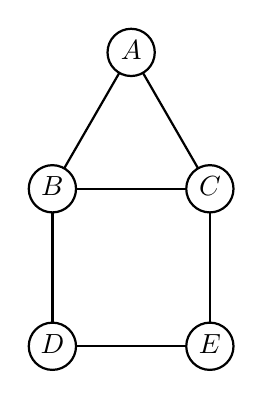
\begin{tikzpicture}[>=latex,thick]
\coordinate (A) at (0,{sqrt(3)});
\coordinate (B) at (-1,0);
\coordinate (C) at (1,0);
\coordinate (D) at (-1,-2);
\coordinate (E) at (1,-2);
\draw[shorten >= 0.3cm,shorten <= 0.3cm] (A) -- (B);
\draw[shorten >= 0.3cm,shorten <= 0.3cm] (A) -- (C);
\draw[shorten >= 0.3cm,shorten <= 0.3cm] (B) -- (C);
\draw[shorten >= 0.3cm,shorten <= 0.3cm] (B) -- (D);
\draw[shorten >= 0.3cm,shorten <= 0.3cm] (C) -- (E);
\draw[shorten >= 0.3cm,shorten <= 0.3cm] (D) -- (E);
\draw (A) circle[radius=0.3];
\draw (B) circle[radius=0.3];
\draw (C) circle[radius=0.3];
\draw (D) circle[radius=0.3];
\draw (E) circle[radius=0.3];
\node at (A) {$A\mathstrut$};
\node at (B) {$B\mathstrut$};
\node at (C) {$C\mathstrut$};
\node at (D) {$D\mathstrut$};
\node at (E) {$E\mathstrut$};
\end{tikzpicture}
\end{center}
\end{loesung}
